\chapter{Connections}\label{ch:connections}
Something about connections

Pointlike $\delta(x-x_\ctxt)$ or distributed $E_\ctxt$
\subsubsection{Alternative interpretation of grid points}
Section \ref{sec:gridFunctions} gives an introduction to how a continuous 1D system is subdivided into grid points in space (see Figure \ref{fig:gridExp}) in a process called discretisation. An alternative way to see grid points after discretisation is shown in Figure \ref{fig:gridExp2}. Rather than grid `points' with a spacing $h$ between them, a continuous system is divided into grid `sections' of width $h$. This interpretation allows the `weight' of a grid point to be calculated from its material properties and geometry. The boundaries have a width of $h/2$ such that the total length $L = Nh$ m.

As an example, the weight of one grid point (or now rather grid section) of a string can be calculated as $\rho A h$. The weight of one grid point of a 2D plane can be calculated as $\rho H h^2$. As these grid points interact with each other, the forces resulting from this interaction are scaled by their respective weight per grid point....

This provides a better intuition for the interactions between components shown in this part. 

\begin{figure}[h]
    \centering
    % \subfloat[If $N=5$ there are 5 sections of length $h$ and 6 grid points describing the state of the system ($l=\{0, \hdots, 5\}$).\label{fig:gridExp1}]{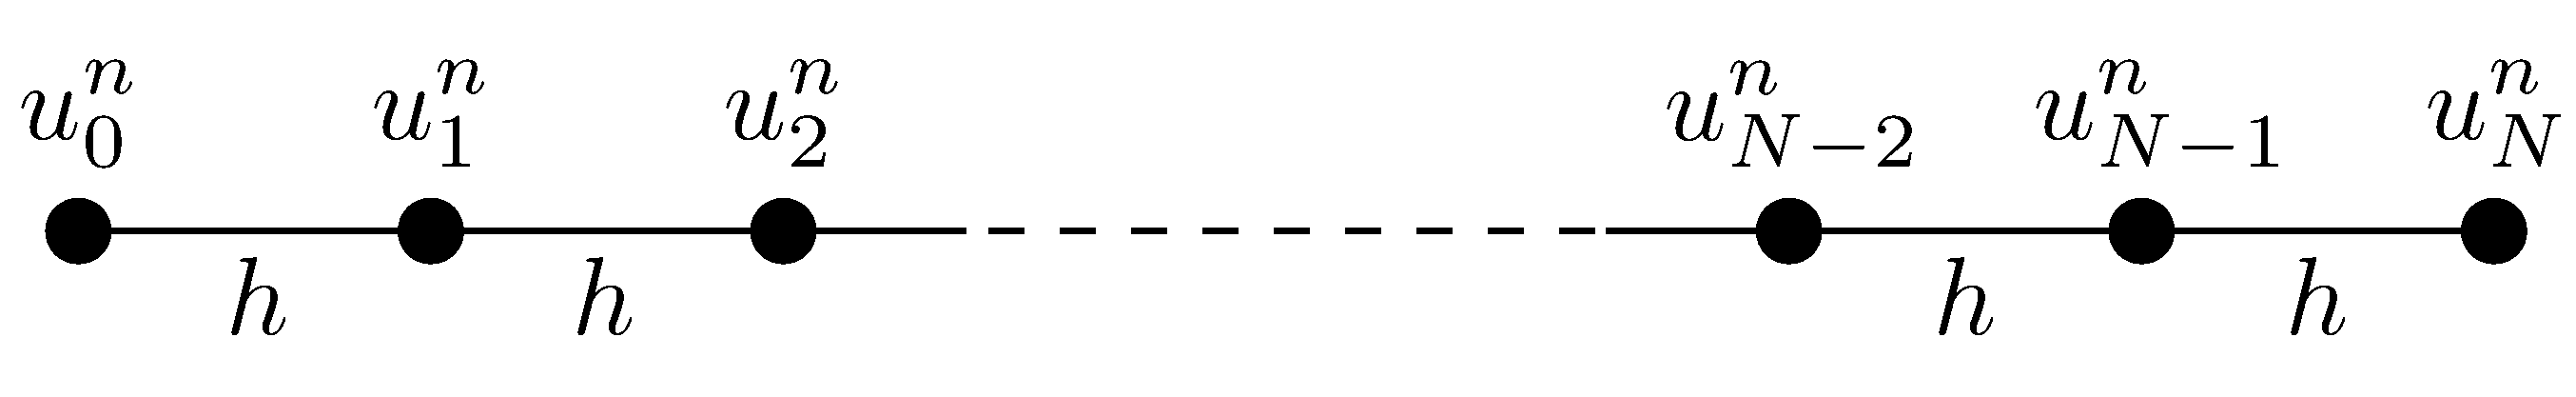
\includegraphics[width=0.45\textwidth]{figures/fdtd/gridExplanation.pdf}}\hspace{0.06\textwidth}
    % \subfloat[If $N$ is large (as is usually the case), The 1D system is divided into $N$ sections of length $h$ and $l=\{0, \hdots, N\}$.\label{fig:gridExp2}]{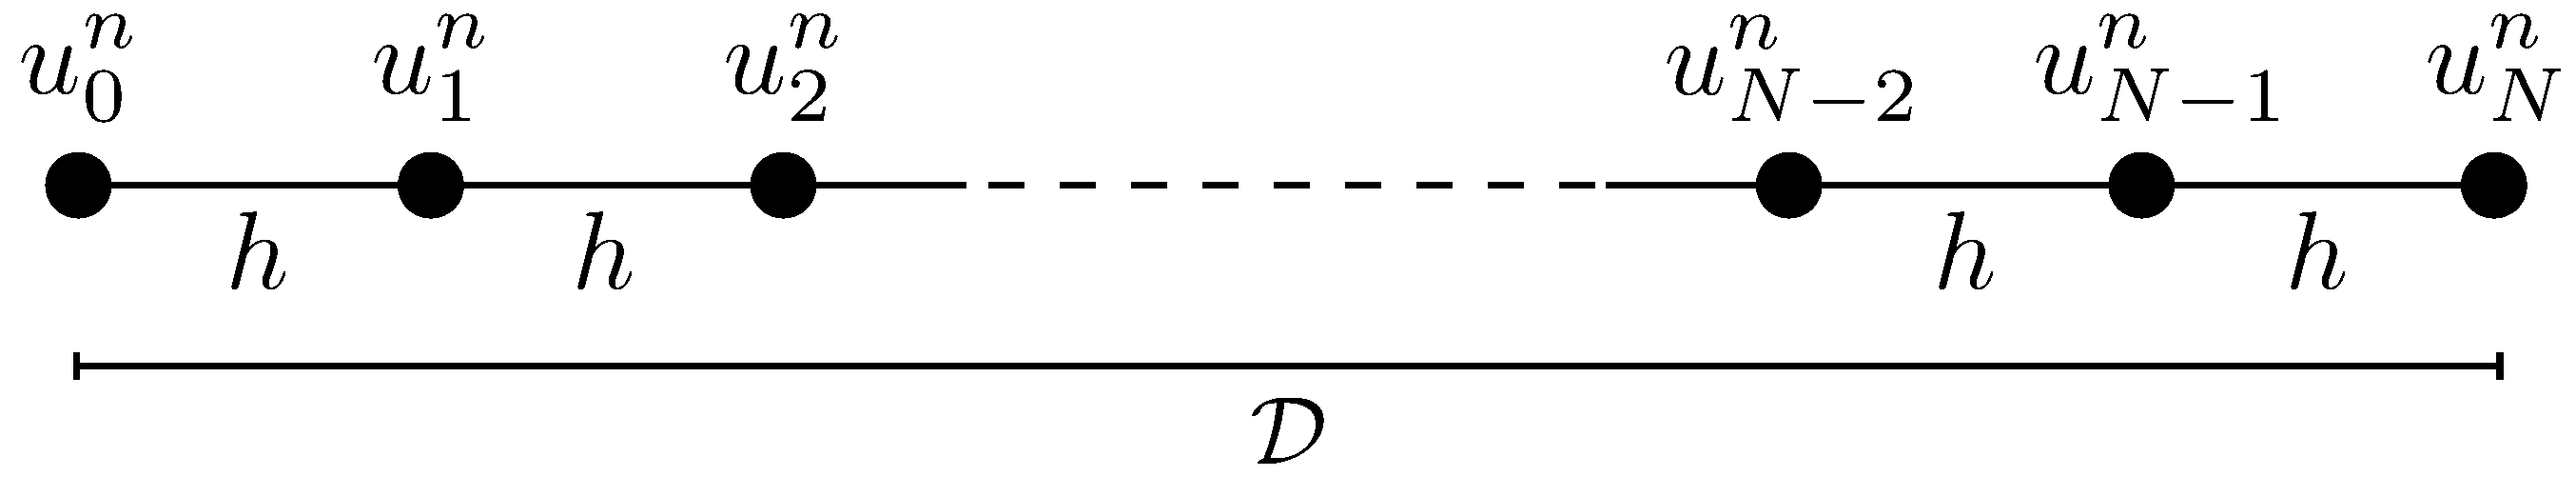
\includegraphics[width=0.45\textwidth]{figures/fdtd/gridExplanation2.pdf}}
    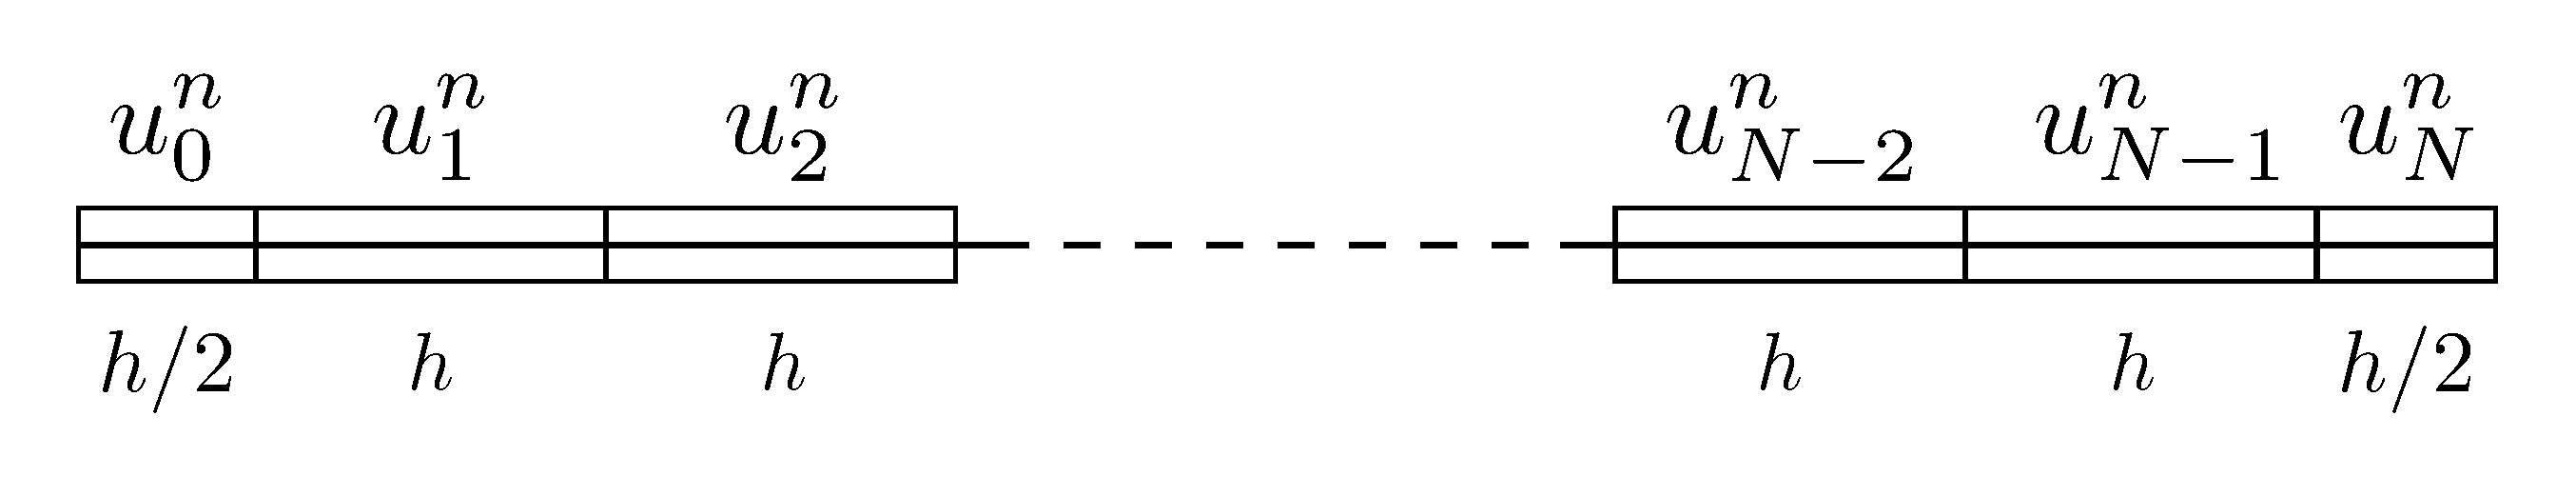
\includegraphics[width=0.75\textwidth]{figures/fdtd/gridFigure2.pdf}
    \caption{Alternative interpretation of the discretisation of $u(x,t)$. The continuous system is divided into $N-1$ sections of width $h$ plus $2$ sections of width $h/2$ at the boundaries. Through this interpretation, the `weight' of a grid point can be calculated from its physical parameters. \label{fig:gridExp2}}
\end{figure}

\section{Rigid connection}
The simplest connection is Forces should be equal and opposite. 

If component $a$ is located `above' component $b$, and their relative displacement is defined as $\eta = a-b$, then a positive $\eta$ is going to have a negative effect on $a$ and a positive effect on $b$ and vice-versa. This is important for the signs when adding the force terms to the schemes. 

\section{Spring-like connections}

\subsection{Connection with rigid barrier (scaled)}
Consider the (scaled) 1D wave equation with an additional force term $F^n$
\begin{equation}\label{eq:1DwaveConnRigid}
    \dtt \uln = \gamma^2\dxx \uln + J(x_\ctxt)F^n
\end{equation}
where
\begin{equation}\label{eq:1DwaveConnRigidForce}
    F^n = -\omega_0^2\mtd\eta^n - \omega_1^4(\eta^n)^2\mtd\eta^n - 2\sigma_\times \dtd \eta^n
\end{equation}
and
\begin{equation}\label{eq:etaRigid}
    \eta^n = I(x_\ctxt)\uln.
\end{equation}

To obtain $F^n$, an inner product of scheme \eqref{eq:1DwaveConnRigid} needs to be taken with $J(x_\ctxt)$ over domain $\D$ which, using identity \eqref{eq:identityIJ} yields 
\begin{equation}\label{eq:1DwaveConnRigidInnerProd}
    \dtt I(x_\ctxt)\uln = \gamma^2 I(x_\ctxt)\dxx \uln + \underbrace{I(x_\ctxt)J(x_\ctxt)}_{\lVert J(x_\ctxt) \rVert^2_\D}F^n.
\end{equation}
As $u$ is connected to a rigid barrier according to \eqref{eq:etaRigid}, a shortcut can be taken and Eqs. \eqref{eq:1DwaveConnRigidForce} and \eqref{eq:etaRigid} can be directly substituted into Eq. \eqref{eq:1DwaveConnRigidInnerProd} to get
\begin{equation}
    \dtt \eta^n = \gamma^2 I(x_\ctxt)\dxx \uln + \lVert J(x_\ctxt)\rVert^2_\D\left( -\omega_0^2\mtd\eta^n - \omega_1^4(\eta^n)^2\mtd\eta^n - 2\sigma_\times \dtd \eta^n\right).
\end{equation}
and solved for $\eta^{n+1}$:
\begin{equation}
    \begin{aligned}
    &\!\!\!\!\!\!\!\!\!\!\!\!\!\!\Big(1 + \lVert J(x_\ctxt)\rVert^2_\D k^2[\omega_0^2/2 + \omega_1^4(\eta^n)^2/2 + \sigma_\times/k] \Big)\eta^{n+1} \\
   = &\ 2 \eta^n - \Big(1 + \lVert J(x_\ctxt)\rVert^2_\D k^2[\omega_0^2/2 + \omega_1^4(\eta^n)^2/2 - \sigma_\times/k]\Big)
    \eta^{n-1}\\
    &+ \gamma^2k^2 I(x_\ctxt)\dxx\uln
    \end{aligned}
\end{equation}
This can then be used to calculate $F^n$ in \eqref{eq:1DwaveConnRigidForce} and can in turn be used to calculate $u_l^{n+1}$ in \eqref{eq:1DwaveConnRigid}.

\subsection{String-plate connection}
In this example, let's consider a string connected to a plate using a nonlinear damped spring. This could be interpreted as a simplified form of how guitar string would be connected to the body. 

\subsubsection{Continuous}
The systems in isolation are as in \eqref{eq:stiffStringPDE} and \eqref{eq:platePDE}, but with an added force term:
\begin{subequations}\label{eq:connStringPlatePDEs}
\begin{align}
    \ptt u &= c^2 \pxx u - \kappa_\stxt^2 \pxxxx u - 2\szX[,\stxt]\pt u + 2\soX[,\stxt] \pt\pxx u - \delta(x-x_\ctxt)\frac{f}{\rho_\stxt A}\\
   \ptt w &= -\kappa_\ptxt^2\Delta\Delta w - 2\szX[,\ptxt]\pt w + 2\soX[,\ptxt] \pt\pxx w + \delta(x-x_\ctxt, y-y_\ctxt)\frac{f}{ \rho_\ptxt H}
\end{align}
\end{subequations}
where
\begin{equation}
    f = f(t) = K_1\eta+K_3\eta^3+R \dot\eta
\end{equation}
and
\begin{equation}
    \eta = \eta(t) = u(x_\ctxt, t) - w(x_\ctxt, y_\ctxt, t)
\end{equation}

\subsubsection{Discrete}
System \eqref{eq:connStringPlatePDEs} can then be discretised as
\begin{align}\label{eq:connStringPlateFDSs}
    \!\!\!\dtt \uln &= c^2 \dxx \uln - \kappa_\stxt^2 \dxxxx \uln - 2\szX[,\stxt]\dtd \uln + 2\soX[,\stxt] \dtm\dxx \uln - J_\stxt(x_\ctxt)\frac{f^n}{\rho_\stxt A}\ ,\\
    \!\!\!\dtt \wln &= -\kappa_\ptxt^2\dTwoD\dTwoD \wln - 2\szX[,\ptxt]\dtd \wln + 2\soX[,\ptxt] \dtm\dxx \wln + J_\ptxt(x_\ctxt, y_\ctxt)\frac{f^n}{ \rho_\ptxt H}\ ,
\end{align}
where
\begin{equation}
    f^n = K_1\mtt\eta^n+K_3(\eta^n)^2\mtd\eta^n+R\dtd\eta^n,
\end{equation}
and
\begin{equation}
    \eta^n = I(x_\ctxt)\uln - I(x_\ctxt, y_\ctxt)\wln.
\end{equation}

\subsubsection{Expansion}
System \eqref{eq:connStringPlateFDSs} can be expanded at the connection location $x_\ctxt$ by taking an inner product of the schemes with their respective spreading operators. 


\subsection{Solving for $f$}


\subsection{Non-dimensional}
The scaled system can be written as:
\begin{align}
    \ptt u &= \gamma^2 \pxx u - \kappa_\stxt^2 \pxxxx u - 2\szX[,\stxt]\pt u + 2\soX[,\stxt] \pt\pxx u - \delta(x-x_\ctxt)F\\
   \pt w &= -\kappa_\ptxt^2\Delta\Delta w - 2\szX[,\ptxt]\pt w + 2\soX[,\ptxt] \pt\pxx w + \delta(x-x_\ctxt, y-y_\ctxt)F
\end{align}
where
\begin{equation}
    F = F(t) = \omega_1^2\eta+\omega_3^4\eta^3+\sigma_\ctxt \dot\eta
\end{equation}
and
\begin{equation}
    \eta = \eta(t) = u(x_\ctxt, t) - w(x_\ctxt, y_\ctxt, t)
\end{equation}


\begin{equation}
    I(x_\ctxt)\delta_{tt}\uln = c^2
    \left(I(x_\ctxt)\dxx\uln\right) + I(x_\ctxt)J(x_\ctxt)F
\end{equation}